\section{Origins of Spelling Checkers and Correctors}

With the emergence of word processing programs and the following digitalization of text documents, spelling checkers and correctors have become a common helper in our everyday lives. However, the research on this topic has begun much earlier \cite{program_check_correction}.

The original motivation for a spelling checker was to find input errors in databases. For example, in \cite{data_correction} the authors aim to find incorrectly spelled names, dates and places in a genealogical database. This is done by computing the frequency of trigrams (three sequential characters) in the source text and based on that the probability of a character given some context, i.e. its adjacent characters. Erroneous words are found by looking at its trigrams. If a word consist of a number of unusual character combinations, it is probably spelled wrongly. However, it is easy to see that this method is not very useful for new, rare or foreign expressions like \texttt{doppelg\"{a}nger} and for typos with high probabilities of being correct. Furthermore the model is limited to the vocabulary used in the text.

These problems were solved by the introduction of dictionaries. A dictionary is a list of correctly spelled words which can optionally be extended by the user. For every word, the program checks if it is part of the dictionary. If it is, then it is spelled correctly, otherwise there is an error.

This method was enhanced by the addition of a spelling corrector. In \cite{dictionary_correction} a dictionary is used to find incorrect words. It is then assumed that these words contain only one of four types of errors: one character was wrong, one extra character was inserted, one character was missing or two adjacent characters were transposed. Under this assumption the dictionary is searched for possible corrections. In \cite{digram_correction} the author uses a dictionary to find incorrect words as well. For the found words he uses digrams (similar to the trigrams mentioned above, just with two instead of three characters) to suggest corrections for incorrect words.

\begin{figure}[t]
\centering
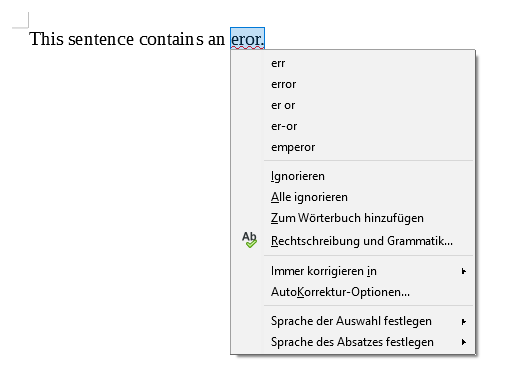
\includegraphics[width=0.9\linewidth]{word_error}
\caption{Screenshot from the LibreOffice Writer program. An example of error correction in a word processing software. The misspelled word is flagged and possible corrections are proposed to the user.}
\label{word_correction}
\end{figure}

The addition of user interaction results in even more convenience. Instead of just outputting a list of incorrect words and corrections, the program would show the user the words it assumed to be incorrectly spelled and then give the user some possible actions to chose from like \texttt{ignore} or \texttt{replace} (compare figure \ref{word_correction}).

\subsection{Modern Research}

Of course the methods described so far do still not take the context of the text into account. For example if \texttt{know} is misspelled as \texttt{now}, no error is indicated even though it could be concluded from the context that a verb is expected in this place. This "context-awareness" has been the topic of a lot of recent research. In \cite{context_n_gram} n-grams are used to determine the most likely replacement for an error and in \cite{context_sensitive_spelling} the authors concentrate on finding and correcting small spelling errors that result in correct words and are therefore not detected by a traditional spelling checker (e.g. \texttt{to} for \texttt{too} or \texttt{there} for \texttt{their}). Other researchers concentrated on a particular set of errors like article \cite{article_correction} or preposition errors \cite{preposition_correction}.

However, even though these methods perform well on the errors they were designed for, a large amount of different classifiers is needed to catch every error. This is a costly and inflexible approach. Recent research often uses statistical machine translation methods or language models and n-grams to correct errors of multiple classes \cite{grammatical_error_task}. In \cite{seq2seq_on_text_correction} the authors train an encoder-decoder neural network with an attention mechanism which operates at the character level. \cite{seq2seq_keyboard} chose a similar approach applied to keyboard decoding on smartphones.

\section{Automatic Correction of Source Code}

Of course automatic error correction is also a useful helper for writing code. Because of the well-defined syntax of a programming language, syntactical errors are relatively easy to find using an algorithm. This functionality can help novice programmers to avoid typical beginner's errors like a missing semicolon at the end of the line. However, semantic and logical errors can usually not be detected this easily.

Of course the correctability of a programming language depends in part on its properties. One important distinction is between strongly typed and weakly typed programming languages \cite{pl_typing}. In a strongly typed programming language, every variable has a fixed type and every method has a fixed return type. This enables an editor program to check if the expected and the actual type match before runtime. This error can then be flagged and shown to the user. In contrast, in a weakly typed programming language, variables don't have a fixed type. They can contain whatever value one assigns to them and similarly methods can take arguments of any type and also return values of any type. In this case, an error of an operation which gets an unexpected parameter type only shows at runtime. For example on the one hand, the type error in

\lstset{belowskip=3mm}
\begin{lstlisting}
public void printNumber(String n){
  System.out.println("Number: " + n);
}
printNumber(9);
\end{lstlisting}

\noindent can be detected before runtime because Java is a strongly typed programming language. The type of the parameter \texttt{n} is defined as \texttt{String} and the method invocation with an argument of type \texttt{int} is clearly wrong. On the other hand the type error in

\lstset{language=Python}
\begin{lstlisting}
def print_number(n):
  print("Number: " + n)
print_number(9)
\end{lstlisting}
\lstset{language=Java}
\lstset{belowskip=0mm}

\noindent shows only at runtime. Python is a weakly typed language and in general it can not be determined of which type a variable is allowed to be before runtime. Only when the code is executed, the \texttt{+} operator looks at its arguments and throws an error if their types don't match.

\begin{figure}[t]
\centering
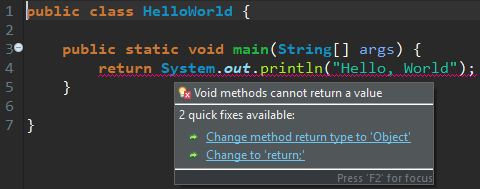
\includegraphics[width=0.9\linewidth]{eclipse_error}
\caption{Screenshot from the Eclipse Java IDE. An example of error correction in an integrated development environment. The erroneous code is flagged and possible quick fixes are proposed to the user.}
\label{ide_correction}
\end{figure}

Early work used the specific properties and grammar of a programming language to develop algorithms which catch errors where ever possible \cite{syntax_correction_in_pl, analysis_for_editors}. Modern integrated development environments (IDEs) still use such algorithms to provide error detection and correction functionality to the programmer (compare figure \ref{ide_correction}).

However, it is impossible for a traditional algorithm to find all errors in a program. Depending on the properties of the programming language it can be hard to find semantic errors and logical errors are even harder to detect because they require an understanding of the purpose of the program. Even a human struggles to detect errors in the logic of a program and that is why a model which is able to find these errors would be very useful.

Because traditional algorithms are insufficient, the attention of recent research has shifted to deep neural networks. In \cite{programming_assignments_correction} the authors train a recurrent neural network model on the task of correcting beginners syntax errors in small programs. They train on a large corpus of student submissions for five simple programming tasks with the purpose of automatically generating feedback for such exercises thus replacing the need of a human to do so. \cite{rnn_syntax_correction} also use a recurrent architecture to predict the exact location of a syntax error and to suggest possible corrections.
